\chapter{Avaliação dos Resultados}
\label{cap:impl}

Para avaliação dos resultados obtidos, foram
selecionados 6 tópicos distribuídos em duas categorias diferentes:
comentários políticos e discussão sobre filmes. Foram escolhidas duas
categorias distintas com o objetivo de avaliar a assertividade dos sentimentos identificados pela ferramenta, sobre
comentários com diferentes tamanhos, contextos e usuários. Para utilização do
Método de Propagação Dupla em conjunto com a extração de sentimentos
relacionados com um único alvo, foram selecionadas as seguintes palavras como
alvo: \textit{``movie''} para os tópicos relacionados a filmes e
\textit{``Trump''} para os tópicos relacionados a política.

No que diz respeito a tópicos relacionados com ao cenário político, os
tópicos escolhidos foram:
\begin{itemize}
  \item
  \textit{Donald Trump to strip all funding from State Dept team promoting
  women's rights around the world - Leaked plan comes as First Daughter Ivanka
  defends her father's record with women}: esse tópico contém 9246
  comentários e encontra-se disponível em
  \url{https://www.reddit.com/r/worldnews/comments/67ivae/donald_trump_to_strip_all_funding_from_state_dept/}
  e refere-se a decisão do presidente dos Estados Unidos da América, Donald
  Trump, em remover fundos de promoção ao direito das mulheres.  
  \item
  \textit{Sweden asks the U.S. to explain Trump comment on
  Sweden}: esse tópico contém 10927
  comentários e encontra-se disponível em
  \url{https://www.reddit.com/r/worldnews/comments/5uzetf/sweden_asks_the_us_to_explain_trump_comment_on/}
  e se refere aos comentários feitos do presidente dos Estados Unidos da
  América, Donald Trump, sobre a Suécia.
  
  \item\textit{“Canada will welcome you,” Trudeau invites refugees as Trump bans
  them}: esse tópico contém 9113
  comentários e encontra-se disponível em
  \url{https://www.reddit.com/r/worldnews/comments/5qqa51/canada_will_welcome_you_trudeau_invites_refugees/}
  e refere-se a declaração do primeiro ministro canadense sobre decisão de
  receber refugiados. Neste declaração, o primeiro ministro canadense afirma que
  os refugiados serão bem-vindos no Canadá.
\end{itemize}

Já os tópicos escolhidos que se referem a discussão sobre filmes são:

\begin{itemize}
  \item
  \textit{Official Discussion - mother! [SPOILERS]}: esse tópico contém 5297
  comentários e encontra-se disponível em
  \url{https://www.reddit.com/r/movies/comments/706y1p/official_discussion_mother_spoilers/}
  e apresenta a avaliação do filme \textit{``Mother!''}.
  \item
  \textit{Official Discussion: Gerald's Game [SPOILERS]}: esse tópico contém 892
  comentários e
  encontra-se disponível em
  \url{https://www.reddit.com/r/movies/comments/73g2fx/official_discussion_geralds_game_spoilers/}
  e apresenta a avaliação do filme \textit{``Gerald's Game''}.
    \item
  \textit{Official Discussion: The Mummy (2017) [SPOILERS]}: esse tópico contém
  1333 comentários e
  encontra-se disponível em
  \url{https://www.reddit.com/r/movies/comments/6g5lmo/official_discussion_the_mummy_2017_spoilers/}
  e apresenta a avaliação do filme \textit{``The Mummy''}.
  
\end{itemize}



\subsection{Uso da Ferramenta para Análise de
Sentimentos na Rede Social Reddit}

A partir da ferramenta desenvolvida, foi realizada a análise dos tópicos
descritos, utilizando um dicionário gerado através do
Método de Propagação Dupla com palavra extraídas de um mesmo tema, e também
foram escolhidas palavras alvo para extração dos comentários e sentimentos
relacionados com elas. A partir deste processo, foram obtidos os seguintes
resultados:

\begin{itemize}
  \item 75\% de assertividade no tópico \textit{Official Discussion - mother!}.
  \item 72,34\% de assertividade no tópico \textit{Official Discussion: Gerald's
  Game}.
  \item 63,04\% de assertividade no tópico \textit{Official Discussion: The
  Mummy}.
  \item 65,21\% de assertividade no tópico \textit{“Canada will welcome you,”
  Trudeau invites refugees as Trump bans them}.
  \item 62,79\% de assertividade no tópico \textit{Donald Trump to strip all
  funding from State Dept team promoting women's rights around the world - Leaked plan comes as First Daughter Ivanka defends her father's record with women}.
  \item 49,49\% de assertividade no tópico \textit{Sweden asks the U.S. to
  explain Trump comment on Sweden}.
\end{itemize}


\begin{figure}[!htbp]
\centering
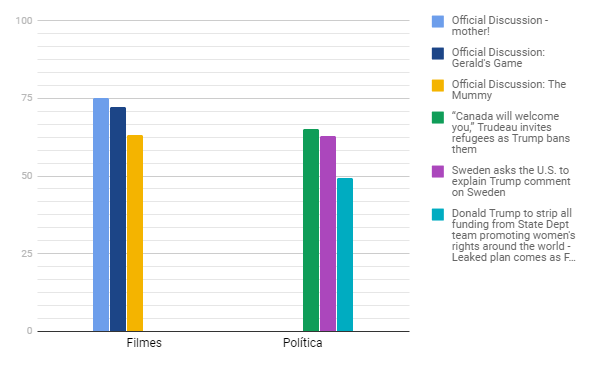
\includegraphics[height=300px]{imagens/grafico1.png}
\caption{Assertividade da ferramenta desenvolvida.}
\label{fig:ass}
\end{figure}

Através dos resultados
apresentados, pode-se verificar que a ferramenta apresentou maior assertividade
ao análisar comentários de filmes aonde o resultado se mostrou similar ao
apresentado por Pålsson e Szerszen
\cite{SentimentinSocialMedia}. 

Em relação aos tópicos relacionados a política, a ferramenta apresentou uma
baixa assertividade, chegando a apresentar assertividade similar a assertividade
obtida por classificando comentários de forma aleatória, o que naturalmente
iria classificar os comentários com 50\% de acerto eventualmente.

\newpage

Destaca-se que os tópicos de discussão de filmes encorajam o leitor a avaliar o
filme que está sendo discutido apresentando uma enquete em seu corpo, enquanto
os comentários sobre política apresentam no conteúdo de seu tópico somente um
\textit{link} direto para a notícia original. 

Como o \ac{VADER} faz uso de um
dicionário para a avaliação dos sentimentos, e nos tópicos relacionados com
política não é pedido que o autor do comentário expresse sua opinião sobre o
que estamos querendo avaliar, o \ac{VADER} acaba atribuindo sentimentos não
existentes ou com sua polaridade errada em determinadas frases, como por
exemplo: 

\textit{``\ldots What if he is just like trump and trump's useless
father\ldots``}. 

Neste caso, o dicionário irá avaliar de forma positiva o
comentário pois a palavra \textit{``like''}, quando utilizada com o significado
de ``gostar'' apresenta um sentimento positivo, porém, a palavra
\textit{``like''} neste caso está sendo utilizada como comparação, fazendo com
que a ferramenta apresente o sentimento errado.
